% THIS DOCUMENT IS TAILORED TO REQUIREMENTS FOR SCIENTIFIC COMPUTING.  IT SHOULDN'T
% BE USED FOR NON-SCIENTIFIC COMPUTING PROJECTS
\documentclass[12pt]{article}

\usepackage{amsmath, mathtools}
\usepackage{amsfonts}
\usepackage{amssymb}
\usepackage{graphicx}
\usepackage{colortbl}
\usepackage{xr}
\usepackage{hyperref}
\usepackage{longtable}
\usepackage{xfrac}
\usepackage{tabularx}
\usepackage{float}
\usepackage{siunitx}
\usepackage{booktabs}
\usepackage{caption}
\usepackage{pdflscape}
\usepackage{afterpage}

\usepackage[round]{natbib}

%\usepackage{refcheck}

\hypersetup{
    bookmarks=true,         % show bookmarks bar?
      colorlinks=true,       % false: boxed links; true: colored links
    linkcolor=red,          % color of internal links (change box color with linkbordercolor)
    citecolor=green,        % color of links to bibliography
    filecolor=magenta,      % color of file links
    urlcolor=cyan           % color of external links
}

%% Comments

\usepackage{color}

\newif\ifcomments\commentstrue %displays comments
%\newif\ifcomments\commentsfalse %so that comments do not display

\ifcomments
\newcommand{\authornote}[3]{\textcolor{#1}{[#3 ---#2]}}
\newcommand{\todo}[1]{\textcolor{red}{[TODO: #1]}}
\else
\newcommand{\authornote}[3]{}
\newcommand{\todo}[1]{}
\fi

\newcommand{\wss}[1]{\authornote{blue}{SS}{#1}} 
\newcommand{\plt}[1]{\authornote{magenta}{TPLT}{#1}} %For explanation of the template
\newcommand{\an}[1]{\authornote{cyan}{Author}{#1}}

%% Common Parts

\newcommand{\progname}{Damped Harmonic Ocsillator} % PUT YOUR PROGRAM NAME HERE
\newcommand{\authname}{
\\ Muhammad Waqar Ul Hassan Awan
} % AUTHOR NAMES                  

\usepackage{hyperref}
    \hypersetup{colorlinks=true, linkcolor=blue, citecolor=blue, filecolor=blue,
                urlcolor=blue, unicode=false}
    \urlstyle{same}
                                


% For easy change of table widths
\newcommand{\colZwidth}{1.0\textwidth}
\newcommand{\colAwidth}{0.13\textwidth}
\newcommand{\colBwidth}{0.82\textwidth}
\newcommand{\colCwidth}{0.1\textwidth}
\newcommand{\colDwidth}{0.05\textwidth}
\newcommand{\colEwidth}{0.8\textwidth}
\newcommand{\colFwidth}{0.17\textwidth}
\newcommand{\colGwidth}{0.5\textwidth}
\newcommand{\colHwidth}{0.28\textwidth}

% Used so that cross-references have a meaningful prefix
\newcounter{defnum} %Definition Number
\newcommand{\dthedefnum}{GD\thedefnum}
\newcommand{\dref}[1]{GD\ref{#1}}
\newcounter{datadefnum} %Datadefinition Number
\newcommand{\ddthedatadefnum}{DD\thedatadefnum}
\newcommand{\ddref}[1]{DD\ref{#1}}
\newcounter{theorynum} %Theory Number
\newcommand{\tthetheorynum}{TM\thetheorynum}
\newcommand{\tref}[1]{TM\ref{#1}}
\newcounter{tablenum} %Table Number
\newcommand{\tbthetablenum}{TB\thetablenum}
\newcommand{\tbref}[1]{TB\ref{#1}}
\newcounter{assumpnum} %Assumption Number
\newcommand{\atheassumpnum}{A\theassumpnum}
\newcommand{\aref}[1]{A\ref{#1}}
\newcounter{goalnum} %Goal Number
\newcommand{\gthegoalnum}{GS\thegoalnum}
\newcommand{\gsref}[1]{GS\ref{#1}}
\newcounter{instnum} %Instance Number
\newcommand{\itheinstnum}{IM\theinstnum}
\newcommand{\iref}[1]{IM\ref{#1}}
\newcounter{reqnum} %Requirement Number
\newcommand{\rthereqnum}{R\thereqnum}
\newcommand{\rref}[1]{R\ref{#1}}
\newcounter{nfrnum} %NFR Number
\newcommand{\rthenfrnum}{NFR\thenfrnum}
\newcommand{\nfrref}[1]{NFR\ref{#1}}
\newcounter{lcnum} %Likely change number
\newcommand{\lthelcnum}{LC\thelcnum}
\newcommand{\lcref}[1]{LC\ref{#1}}

\usepackage{fullpage}

\newcommand{\deftheory}[9][Not Applicable]
{
\newpage
\noindent \rule{\textwidth}{0.5mm}

\paragraph{RefName: } \textbf{#2} \phantomsection 
\label{#2}

\paragraph{Label:} #3

\noindent \rule{\textwidth}{0.5mm}

\paragraph{Equation:}

#4

\paragraph{Description:}

#5

\paragraph{Notes:}

#6

\paragraph{Source:}

#7

\paragraph{Ref.\ By:}

#8

\paragraph{Preconditions for \hyperref[#2]{#2}:}
\label{#2_precond}

#9

\paragraph{Derivation for \hyperref[#2]{#2}:}
\label{#2_deriv}

#1

\noindent \rule{\textwidth}{0.5mm}

}

\begin{document}

\title{Software Requirements Specification for \progname:
Damped Harmonic Oscillator Illustrated by Online Calculator} 
\author{\authname}
\date{\today}
	
\maketitle

~\newpage

\pagenumbering{roman}

\tableofcontents

~\newpage

\section*{Revision History}

\begin{tabularx}{\textwidth}{p{3cm}p{2cm}X}
\toprule {\bf Date} & {\bf Version} & {\bf Notes}\\
\midrule
February 2, 2024 & 1.0 & Initial Document Release\\
\bottomrule
\end{tabularx}

~\newpage

\section{Reference Material}

This section records information for easy reference.

\subsection{Table of Units}

Throughout this document SI (Syst\`{e}me International d'Unit\'{e}s) is employed
as the unit system.  In addition to the basic units, several derived units are
used as described below.  For each unit, the symbol is given followed by a
description of the unit and the SI name.
~\newline

\renewcommand{\arraystretch}{1.2}
%\begin{table}[ht]
  \noindent \begin{longtable*}{l l l}
    \toprule		
    \textbf{symbol} & \textbf{unit} & \textbf{SI}\\
    \midrule 
    \si{\metre} & length & metre\\
    \si{\kilogram} & mass	& kilogram\\
    \si{\second} & time & second\\
    \si{\newton} & force & Newton\\
    \si{\hertz} & frequency & hertz (\si{\second^{-1}})\\
    v & velocity & metre per second (\si{\meter\per\second})\\
    a & acceleration & metre per second square (\si{\meter\per\square\second})\\
    g & gravity & metre per second square (\si{\meter\per\square\second})\\
    \bottomrule
  \end{longtable*}
  %	\caption{Provide a caption}
%\end{table}

\subsection{Table of Symbols}

The table that follows summarizes the symbols used in this document along with
their units.  The choice of symbols was made to be consistent with the heat
transfer literature and with existing documentation for solar water heating
systems.  The symbols are listed in alphabetical order.

\renewcommand{\arraystretch}{1.2}
%\noindent \begin{tabularx}{1.0\textwidth}{l l X}
\noindent \begin{longtable*}{l l l} \toprule
\textbf{symbol} & \textbf{unit} & \textbf{description}\\
\midrule 
$k$ & Newton per metre (\si{\newton\per\metre}) & Spring Constant\\
$c$ & kilogram per second (\si{\kilogram\per\second}) & Damping Coefficient\\
$x$ & metre (\si{\metre}) & Displacement\\
$w$ & radians per second (\si{\radian\per\second}) & Angular Frequency\\
\bottomrule
\end{longtable*}

\newpage

\subsection{Abbreviations and Acronyms}

\renewcommand{\arraystretch}{1.2} 
\begin{longtable*}{l l}
  \toprule		
  \textbf{symbol} & \textbf{description}\\
  \midrule 
  SRS & Software Requirement Specification\\
  ODE & Ordinary Differential Equation\\
  DE & Differential Equation\\
  DHO & Damped Harmonic Oscillator\\
  SHM & Simple Harmonic Motion\\
  \bottomrule
\end{longtable*}

\subsection{Mathematical Notation}

\begin{itemize}
  \item \textbf{Greek symbols} represent constants and parameters, such as $\omega$ for angular frequency.
  \item \textbf{Subscripts} are used to denote specific instances or components, e.g., $x_{t}$ for the position at time t.
  \item \textbf{Mathematical operations} and functions are denoted as follows: $sin$ and $cos$ for trigonometric functions, $e$ for the exponential function, and $d/dt$ for differentiation with respect to time.
\end{itemize}

\newpage

\section{Introduction}

In physics and engineering, the concept of harmonic oscillators gives 
us a way to understand how things move back and forth or oscillate. It 
offering insights into systems' behavior under periodic forces. 
Understanding system dynamics of a simple pendulum or a mass attached 
to a spring is crucial for advancements in various scientific and 
engineering fields. This document introduces a software project aimed 
at modeling and analyzing harmonic oscillators, providing a tool for 
educational, research, and industrial applications to observe the effect 
of damping on oscillating bodies.
\newline
\newline
This introduction serves as a roadmap to the document, outlining its 
structure and guiding the reader through the subsequent sections. 
Following this introduction, the document details the purpose of the 
SRS, the scope of requirements, characteristics of the intended reader, 
and the organization of the document itself.

\subsection{Purpose of Document}

The purpose of this Software Requirement Specification (SRS) document 
is to outline the functional and non-functional requirements for a 
software project focused on the simulation and analysis of harmonic 
oscillators. This document is intended to serve as a comprehensive 
guide for the development team, ensuring that the software meets the 
specific needs of its users. Additionally, this SRS aims to facilitate 
clear communication among stakeholders, provide a basis for estimating 
costs and timelines, and implementation phases of the project.

\subsection{Scope of Requirements} 

This project is the simulation of harmonic oscillators, a fundamental 
concept in physics. To manage the complexity in modeling real-world 
phenomena, the scope of this software will be constrained. Specifically, 
the project will focus on:

\begin{itemize}
  \item Modeling in two dimensions to simplify visualizations and 
  computations.
  \item Ignoring environmental factors such as temperature and pressure 
  variations that might affect the system's properties.
\end{itemize}

These constraints are chosen to make the problem tractable while still 
providing valuable insights and educational utility.

\subsection{Characteristics of Intended Reader} \label{sec_IntendedReader}

This document is written for the people who will help build, review, 
and maintain the software. They should know their way around basic 
physics and be comfortable with the mathematics, especially the 
oscillators and how they work. They don't need to be physicists, but 
they should understand the science behind what I am trying to simulate.

\subsection{Organization of Document}

The document is organized to facilitate easy navigation and understanding 
of the software requirements. After this section, the document is structured 
as follows:

\begin{itemize}
  \item Section 3: General System Description
  \item Section 4: Specific System Description
  \item Section 5: Requirements
\end{itemize}

Readers are encouraged to refer to Section 3 for general system description, 
Section 4 for specific system description, and Section 5 for requirements.

\section{General System Description}

This section outlines the overall framework of the software designed to 
simulate and analyze harmonic oscillators, both simple and damped. It aims 
to provide a basic understanding of how the system interacts with 
its environment, detailing user interaction, external interfaces, and 
inherent system constraints. The purpose here is to establish a broad 
context that will make the specific requirements outlined in subsequent 
sections clearer and more meaningful. By describing the system at a general 
level, this section remains applicable even as specific functionalities 
evolve or expand within the project's scope.

\subsection{System Context}

The software operates on a basic design pattern of Inputs → Calculations 
→ Outputs, facilitating user interaction through a structured and intuitive 
interface. Users input parameters related to the harmonic oscillator system, 
such as mass, damping coefficients, spring constants, initial conditions, 
and time frames for simulation. The software processes these inputs to 
perform complex calculations, simulating the oscillator's behavior over 
time. The calculated data is then formatted into outputs that are meaningful 
to the user, such as displacement, velocity, energy over time, and 
visualizations of the oscillator's motion.

\begin{figure}[h!]
\begin{center}
 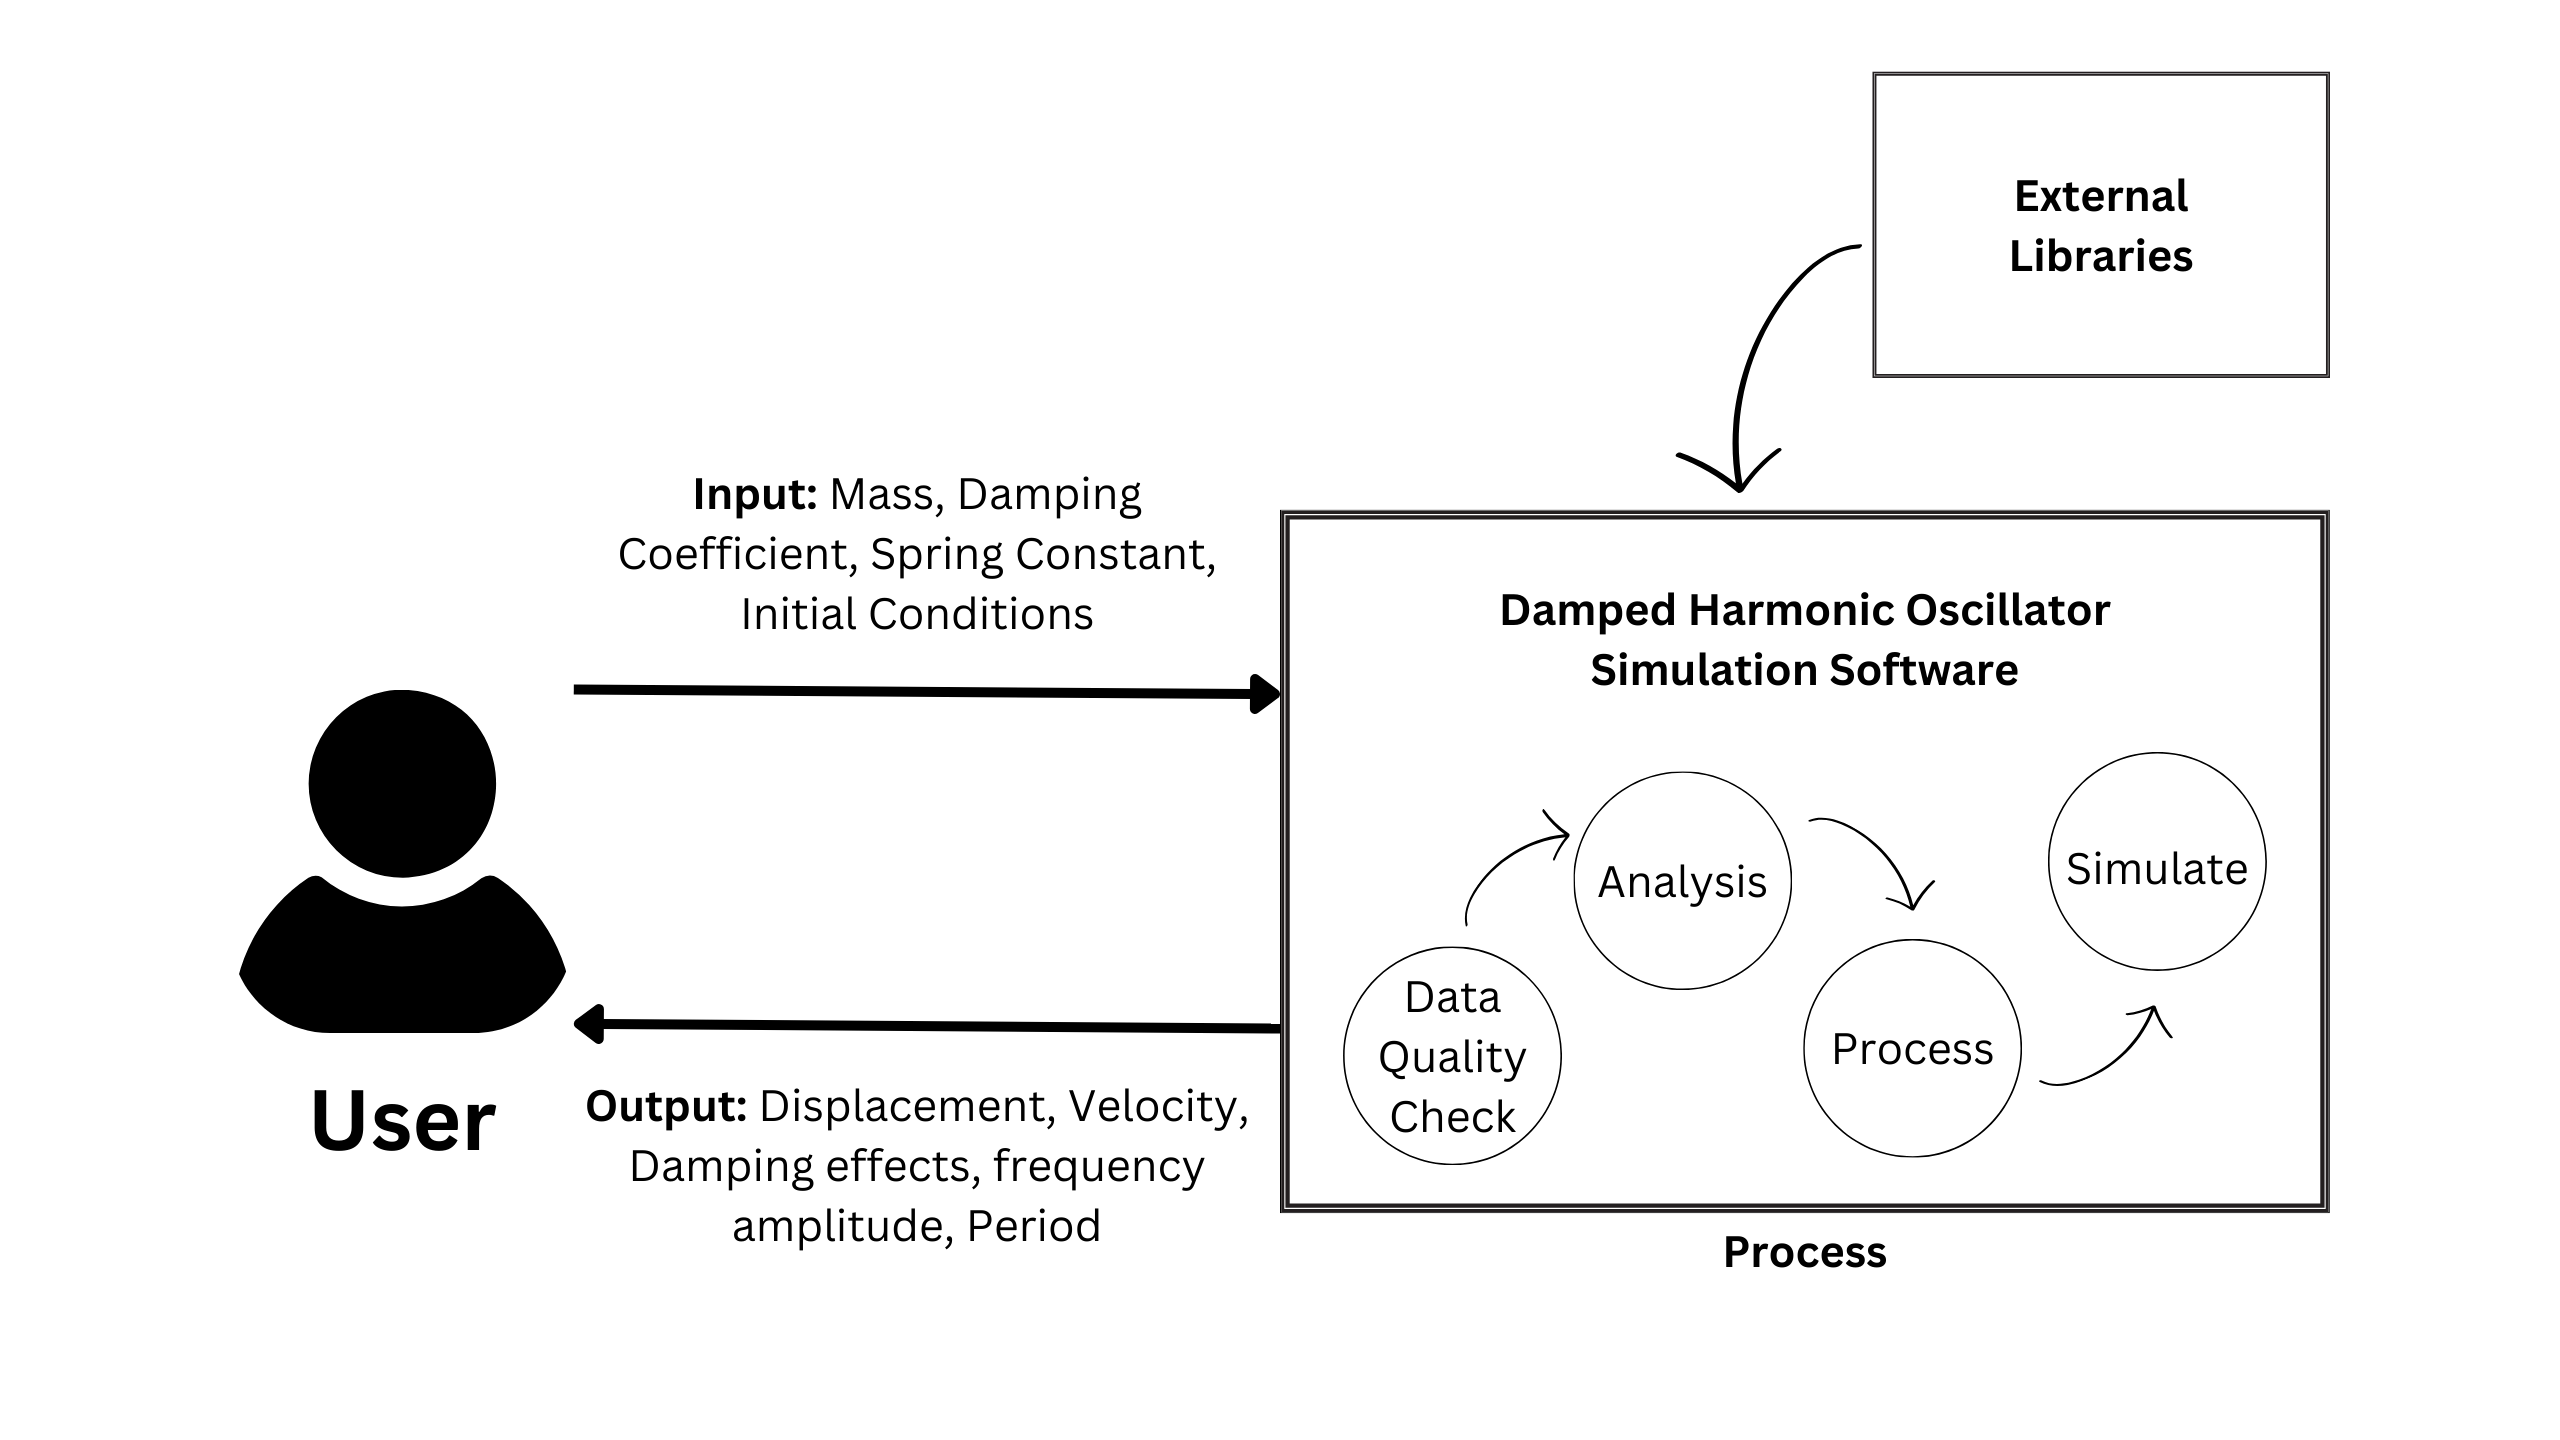
\includegraphics[width=0.8\textwidth]{./systemContext.png}
\caption{System Context}
\label{Fig_SystemContext} 
\end{center}
\end{figure}

\begin{itemize}
\item User Responsibilities:
  \begin{itemize}
  \item Provide accurate and complete input data relevant to the harmonic 
  oscillator being analyzed, including material properties, system geometry, 
  initial conditions, and any external forces or constraints.
  \item Interpret the outputs generated by the software, applying them 
  appropriately in their context of use, whether it be for educational, 
  scientific research, engineering analysis, or exploration purposes.
  \end{itemize}
\item \progname{} Responsibilities:
  \begin{itemize}
  \item Accurately process user inputs to simulate the behavior of harmonic 
  oscillators under specified conditions.
  \item Detect and handle data type mismatches (e.g., rejecting non-numeric 
  inputs where numbers are expected) and other input errors.
  \item Generate and present outputs in a clear, understandable format, 
  including graphical visualizations, data tables, and summary reports.
  \item Ensure the software's calculations and outputs maintain high accuracy 
  and reliability, especially in contexts where precision is critical.
  \end{itemize}
\end{itemize}

\subsubsection*{Context of Use:}

The software is designed for use in a variety of contexts, including educational 
environments for teaching physics principles, research settings for exploring 
the dynamics of new materials or mechanical systems, and engineering projects 
requiring precise analysis of oscillatory systems. While the software is robust 
and designed for high accuracy, its application to mission-critical or 
safety-critical systems should be approached with caution, ensuring that all 
inputs are verified and that outputs are double-checked against other sources 
of analysis where possible.

\subsection{User Characteristics} \label{SecUserCharacteristics}

Users of the Damped Harmonic Oscillator software are expected to have a basic 
understanding of calculus and physics at an undergraduate level. Specifically, 
they should be familiar with the concepts of differential equations as they 
apply to motion and be able to apply basic physics principles to interpret 
the simulation results. This foundational knowledge is crucial for effective 
interaction with the software, enabling users to input realistic parameters 
and accurately interpret simulation outcomes.

\subsection{System Constraints}

Several key constraints influence the design and deployment of this software:

\begin{itemize}
  \item Platform Independence: It should run on common operating systems and 
  web browsers without special hardware requirements.
  \item Libraries and APIs: Where applicable, the software will rely on standard, 
  open-source libraries for mathematical computations and graphical displays 
  (e.g., NumPy, Matplotlib). The choice of these libraries is constrained by 
  their availability, documentation, and compatibility with the target operating 
  systems.
  \item User Interface: Aimed at users with a basic understanding of physics and 
  calculus, the software interface will prioritize simplicity to facilitate 
  learning and exploration without overwhelming users with unnecessary complexity.
\end{itemize}

\section{Specific System Description}

This section delves into the high-level overview of the problem that the Damped 
Harmonic Oscillator software aims to solve. Following this, the solution 
characteristics specification elaborates on the assumptions, theories, definitions, 
and instance models that explains the solution proposed by this project.

\subsection{Problem Description} \label{Sec_pd}

\progname{} targets the problem of accurately modeling and simulating the behavior 
of a damped harmonic oscillator. Such systems are essential in understanding 
phenomena where an object oscillates and gradually loses energy due to resistance 
or damping forces. This simulation is vital in fields such as mechanical 
engineering, where understanding the damping of oscillatory systems can lead to 
better designs and predictions.

\subsubsection{Terminology and  Definitions}

This subsection provides a list of terms that are used in the subsequent
sections and their meaning, with the purpose of reducing ambiguity and making 
it easier to correctly understand the requirements:

\begin{itemize}

\item \textbf{Isolated System:} Neglects external forces other than the damping 
and restoring forces.
\item \textbf{Harmonic Motion:} Assumes that in the absence of damping, the system 
would exhibit simple harmonic motion.
\item \textbf{Linear Damping:} A damping force that is directly proportional to 
the velocity of the oscillating object.
\item \textbf{Nonlinear Damping:} A damping force that varies with velocity in a 
non-proportional manner, often depending on the velocity's magnitude or other factors.

\end{itemize}

\subsubsection{Physical System Description} \label{sec_phySystDescrip}

The system comprises key elements crucial for its analysis and simulation:
\begin{itemize}
  \item \textbf{Mass (m):} Represents the inertia of the oscillating object.
  \item \textbf{Spring Constant (k):} Indicates the force needed to displace the 
  system from its equilibrium position.
  \item \textbf{Damping Coefficient (b):} For linear damping, quantifies the 
  proportionality between the damping force and velocity.
  \item \textbf{Damping Function (f(v)):} For nonlinear damping, represents the 
  relationship between damping force and velocity, which may vary based on the 
  system's specific characteristics.
\end{itemize}
 
 
The system's behavior is significantly influenced by the nature of the damping 
force. The model must account for both linear and nonlinear damping scenarios, 
with the interactions between the mass, spring constant, and damping forces 
defining the system's dynamic response.

% \plt{A figure here makes sense for most SRS documents}

\begin{figure}[h!]
\begin{center}
%\rotatebox{-90}
{
 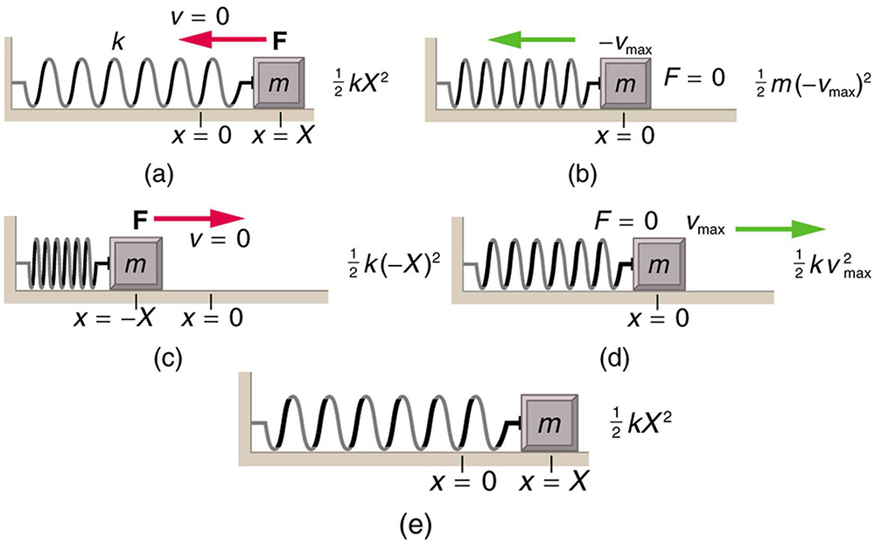
\includegraphics[width=0.5\textwidth]{./physical_system_description.jpg}
}
\caption{Physical System Description}
\end{center}
\end{figure}

\subsubsection{Goal Statements}

With the inclusion of both linear and nonlinear damping forces, the software aims 
to:

\begin{itemize}

  \item[GS\refstepcounter{goalnum}\thegoalnum \label{GS1}:] Create a simulation model that accurately represents the 
  behaviour of a damped harmonic oscillator in various scenarios.
  \item[GS\refstepcounter{goalnum}\thegoalnum \label{GS2}:] Facilitate the understanding of damping effects on 
  oscillatory systems through interactive and visual tools.
  \item[GS\refstepcounter{goalnum}\thegoalnum \label{GS3}:] Simulate of mathematical derivation.
  \item[GS\refstepcounter{goalnum}\thegoalnum \label{GS4}:] Design tools to allow users to create custom scenarios and 
  do comparative analysis. 
  \item[GS\refstepcounter{goalnum}\thegoalnum \label{GS5}:] Enhance educational understanding of damped oscillatory 
  systems.
  
\end{itemize}

\subsection{Solution Characteristics Specification}

This section elaborates on the mathematical and physical principles that form 
the basis of the solution, including assumptions, theoretical models, general 
definitions, and the derivation of instance models.

\subsubsection{Assumptions} \label{sec_assumpt}

This section simplifies the original problem and helps in developing the
theoretical model by filling in the missing information for the physical system.
The numbers given in the square brackets refer to the theoretical model [TM],
general definition [GD], data definition [DD], instance model [IM], or likely
change [LC], in which the respective assumption is used.

\begin{itemize}
\item[A\refstepcounter{assumpnum}\theassumpnum \label{A1}:]
\textbf{Constant Mass [DD2]:} The mass (m) of the oscillator is constant throughout the motion.
\item[A\refstepcounter{assumpnum}\theassumpnum \label{A2}:]
\textbf{Homogeneous Medium [TM:EOM-LDHO, TM:EOM-NDHO]:} Assumes the oscillator moves through a homogeneous medium, affecting the damping forces uniformly across the system.
\item[A\refstepcounter{assumpnum}\theassumpnum \label{A3}:]
\textbf{No External Forces [TM:EOM-LDHO,TM:EOM-NDHO]:} External forces, other 
than damping and restoring forces, are neglected.
\item[A\refstepcounter{assumpnum}\theassumpnum \label{A4}:]
\textbf{Initial Conditions Known [IM1,IM2]:} The initial position and velocity of the oscillator are known and specified.
\end{itemize}

\subsubsection{Theoretical Models}\label{sec_theoretical}

Theoretical models provide the mathematical foundation necessary for understanding and solving the dynamics of damped harmonic oscillators. These models incorporate physical laws and constitutive equations that describe how the system behaves under various conditions, including both linear and non-linear damping forces. The models are crucial for predicting system behavior and formulating solutions that can be applied in practical scenarios.

~\newline

\noindent
\deftheory
% #2 refname of theory
{TM:EOM-LDHO}
% #3 label
{Equation of Motion for Linearly Damped Harmonic Oscillators}
% #4 equation
{
  \begin{equation*}
    m*d\textsuperscript{2}x/dt\textsuperscript{2} + c*dx/dt + kx = 0
  \end{equation*}
}
% #5 description
{
  This equation models the motion of a damped harmonic oscillator, where $m$ is the mass of the oscillator, 
  $dx/dt$, $d\textsuperscript{2}x/dt\textsuperscript{2}$ represent the velocity and acceleration, respectively, 
  $c$ is the damping coefficient for linear damping, $k$ is the spring constant.
}
% #6 Notes
{
  None.
}
% #7 Source
{
  None
}
% #8 Referenced by
{
  \dref{GD1}, \iref{IM1}, \aref{A1}, \aref{A2}, \aref{A3}
}
% #9 Preconditions
{
  Assumes that the oscillator is subject to a restoring force proportional to displacement $x$ from equilibrium and a damping force that is linearly proportional to velocity.
}
% #1 derivation - not applicable by default
{}

\deftheory
% #2 refname of theory
{TM:EOM-NDHO}
% #3 label
{Equation of Motion for Non-Linearly Damped Harmonic Oscillators}
% #4 equation
{
  \begin{equation*}
    m*d\textsuperscript{2}x/dt\textsuperscript{2} + f(dx/dt) + kx = 0
  \end{equation*}
}
% #5 description
{
  This equation models the motion of a damped harmonic oscillator, where $m$ is the mass of the oscillator, 
  $dx/dt$, $d\textsuperscript{2}x/dt\textsuperscript{2}$ represent the velocity and acceleration, respectively, 
  $f(dx/dt)$ represents the function describing non-linear damping forces, $k$ is the spring constant.
}
% #6 Notes
{
  None.
}
% #7 Source
{
  None
}
% #8 Referenced by
{
  \dref{GD1}, \iref{IM1}, \aref{A1}, \aref{A2},\aref{A3}
}
% #9 Preconditions
{
  Assumes that the oscillator is subject to a restoring force proportional to displacement $x$ from equilibrium and a damping force that follows non-linear relationship.
}
% #1 derivation - not applicable by default
{}

~\newline

\subsubsection{General Definitions}\label{sec_gendef}

This section collects the laws and equations that will be used in building the
instance models.

~\newline

\noindent
\begin{minipage}{\textwidth}
\renewcommand*{\arraystretch}{1.5}
\begin{tabular}{| p{\colAwidth} | p{\colBwidth}|}
\hline
\rowcolor[gray]{0.9}
Number& GD\refstepcounter{defnum}\thedefnum\label{GD1}\\
\hline
Label &\bf Damping Force \\
\hline
% Units&$MLt^{-3}T^0$\\
% \hline
SI Units&\si{\newton}(Newton)\\
\hline
Equation& 
$ 
F\textsubscript{damping}=-c*dx/dt 
$ -- Linear Damping
\newline
$ 
F\textsubscript{damping}=-f(dx/dt)
$ -- Non-Linear Damping
\\
\hline
Description &
This definition differentiates between the damping forces in linear and 
non-linear systems. For linear systems, the force is proportional to the 
velocity$(dx/dt)$ with a constant$c$. In contrast, non-linear systems 
exhibit a damping force represented by $f(dx/dt)$, indicating a dependency 
on the velocity's magnitude or other factors.
\\
\hline
  Source & Hadley, Mark. "Damped Harmonic Oscillator" Department of Physics, Graz University of Technology \\
  \hline
  Ref.\ By & \ddref{DD1}, \ddref{DD5}\\
  \hline
\end{tabular}
\end{minipage}\\

~\newline

\noindent
\begin{minipage}{\textwidth}
\renewcommand*{\arraystretch}{1.5}
\begin{tabular}{| p{\colAwidth} | p{\colBwidth}|}
\hline
\rowcolor[gray]{0.9}
Number& GD\refstepcounter{defnum}\thedefnum\label{GD2}\\
\hline
Label &\bf Natural Frequency of Oscillation \\
\hline
% Units&$MLt^{-3}T^0$\\
% \hline
SI Units&\si{\hertz}(Hertz)\\
\hline
Equation& 
$ 
\omega\textsubscript{0}=\sqrt{k/m} 
$
\\
\hline
Description &
This equation provides the natural frequency$(w\textsubscript{0})$ of an 
undamped harmonic oscillator, derived from the spring constant$(k)$ and 
mass$(m)$. It signifies the oscillator's inherent vibrational frequency 
absent damping forces.
\\
\hline
  Source & Hadley, Mark. "Damped Harmonic Oscillator" Department of Physics, Graz University of Technology \\
  \hline
  Ref.\ By & \ddref{DD2}, \ddref{DD3}\\
  \hline
\end{tabular}
\end{minipage}\\

~\newline

\noindent
\begin{minipage}{\textwidth}
\renewcommand*{\arraystretch}{1.5}
\begin{tabular}{| p{\colAwidth} | p{\colBwidth}|}
\hline
\rowcolor[gray]{0.9}
Number& GD\refstepcounter{defnum}\thedefnum\label{GD3}\\
\hline
Label &\bf Energy Dissipation \\
\hline
% Units&$MLt^{-3}T^0$\\
% \hline
SI Units&\si{\joule}(Joules)\\
\hline
Equation& 
\textbf{Total Energy:} $ 
E=1/2*kx^{2}+1/2*mv^{2}
$
\newline
\textbf{Linear Damping Dissipation Rate:} $ 
dE/dt=-c*dx/dt
$
\newline
\textbf{Non-Linear Damping:} Energy Dissipation rate varies with $ 
f(dx/dt) 
$
\\
\hline
Description &
Outlines how the oscillator's total mechanical energy is influenced by 
damping. In linear damping scenarios, energy dissipation is directly 
proportional to the square of velocity, while in non-linear scenarios, 
it is dictated by a function of velocity, $f(dx/dt)$.
\\
\hline
  Source & Hadley, Mark. "Damped Harmonic Oscillator" Department of Physics, Graz University of Technology \\
  \hline
  Ref.\ By & \ddref{DD1}, \ddref{DD2}, \ddref{DD3}, \ddref{DD5}\\
  \hline
\end{tabular}
\end{minipage}\\

\subsubsection{Data Definitions}\label{sec_datadef}

This section collects and defines all the data needed to build the instance
models. The dimension of each quantity is also given.

~\newline

\noindent
\begin{minipage}{\textwidth}
\renewcommand*{\arraystretch}{1.5}
\begin{tabular}{| p{\colAwidth} | p{\colBwidth}|}
\hline
\rowcolor[gray]{0.9}
Number& DD\refstepcounter{datadefnum}\thedatadefnum\label{DD1}\\
\hline
Label& \bf Damping Coefficient\\
\hline
Symbol & $c$ (linear damping), $f(dx/dt)$ (non-linear damping)\\
\hline
% Units& $Mt^{-3}$\\
% \hline
  SI Units & \si{\kilogram\per\second}\\
  \hline
  Equation& -\\
  \hline
  Description & 
  For linear damping, $c$ represents the constant proportionality factor 
  between the damping force and the velocity of the oscillator. For 
  non-linear damping, $f(dx/dt)$ represents a function defining the 
  relationship between the damping force and the velocity, which varies 
  with the velocity's magnitude or other system-specific factors.
  \\
  \hline
  Sources& "Damped Harmonic Oscillator" -- Wikipedia \\
  \hline
  Ref.\ By & \dref{GD1}, \iref{IM1}, \iref{IM2}\\
  \hline
\end{tabular}
\end{minipage}\\

~\newline

\noindent
\begin{minipage}{\textwidth}
\renewcommand*{\arraystretch}{1.5}
\begin{tabular}{| p{\colAwidth} | p{\colBwidth}|}
\hline
\rowcolor[gray]{0.9}
Number& DD\refstepcounter{datadefnum}\thedatadefnum\label{DD2}\\
\hline
Label& \bf Mass\\
\hline
Symbol & $m$\\
\hline
% Units& $Mt^{-3}$\\
% \hline
  SI Units & \si{\kilogram}\\
  \hline
  Equation& -\\
  \hline
  Description & 
  Represents the mass of the harmonic oscillator. The mass is a crucial 
  parameter in determining the system's natural frequency and the dynamics 
  of its motion under damping forces.
  \\
  \hline
  Sources& "Damped Harmonic Oscillator" -- Wikipedia \\
  \hline
  Ref.\ By & \dref{GD2}, \iref{IM1}, \iref{IM2}\\
  \hline
\end{tabular}
\end{minipage}\\

~\newline

\noindent
\begin{minipage}{\textwidth}
\renewcommand*{\arraystretch}{1.5}
\begin{tabular}{| p{\colAwidth} | p{\colBwidth}|}
\hline
\rowcolor[gray]{0.9}
Number& DD\refstepcounter{datadefnum}\thedatadefnum\label{DD3}\\
\hline
Label& \bf Spring Constant\\
\hline
Symbol & $k$\\
\hline
% Units& $Mt^{-3}$\\
% \hline
  SI Units & \si{\newton\per\metre}\\
  \hline
  Equation& -\\
  \hline
  Description & 
  The spring constant $k$ quantifies the stiffness of the spring in the 
  harmonic oscillator. It is a key factor in defining the natural 
  frequency of the oscillator and its response to applied forces.
  \\
  \hline
  Sources& "Damped Harmonic Oscillator" -- Wikipedia \\
  \hline
  Ref.\ By & \dref{GD2}, \iref{IM1}, \iref{IM2}\\
  \hline
\end{tabular}
\end{minipage}\\

~\newline

\noindent
\begin{minipage}{\textwidth}
\renewcommand*{\arraystretch}{1.5}
\begin{tabular}{| p{\colAwidth} | p{\colBwidth}|}
\hline
\rowcolor[gray]{0.9}
Number& DD\refstepcounter{datadefnum}\thedatadefnum\label{DD4}\\
\hline
Label& \bf Natural Frequency\\
\hline
Symbol & $\omega_{0}$\\
\hline
% Units& $Mt^{-3}$\\
% \hline
  SI Units & \si{\radian\per\second}\\
  \hline
  Equation& -\\
  \hline
  Description & 
  The natural frequency $\omega_{0}$ of an undamped harmonic oscillator 
  is determined by its mass $m$ and spring constant $k$. This frequency 
  is foundational for analyzing the oscillator's behavior in the absence 
  of damping forces.
  \\
  \hline
  Sources& "Damped Harmonic Oscillator" -- Wikipedia \\
  \hline
  Ref.\ By & \dref{GD2}\\
  \hline
\end{tabular}
\end{minipage}\\

~\newline

\noindent
\begin{minipage}{\textwidth}
\renewcommand*{\arraystretch}{1.5}
\begin{tabular}{| p{\colAwidth} | p{\colBwidth}|}
\hline
\rowcolor[gray]{0.9}
Number& DD\refstepcounter{datadefnum}\thedatadefnum\label{DD5}\\
\hline
Label& \bf Displacement\\
\hline
Symbol & $x$\\
\hline
% Units& $Mt^{-3}$\\
% \hline
  SI Units & \si{\metre}\\
  \hline
  Equation& -\\
  \hline
  Description & 
  Displacement $x$ from the equilibrium position provides a measure of 
  how far the oscillator moves over time. It is a fundamental quantity 
  for describing the oscillator's motion and is affected by both damping 
  forces and the system's natural dynamics.from the equilibrium position 
  provides a measure of how far the oscillator moves over time. It is a 
  fundamental quantity for describing the oscillator's motion and is 
  affected by both damping forces and the system's natural dynamics.
  \\
  \hline
  Sources& "Damped Harmonic Oscillator" -- Wikipedia \\
  \hline
  Ref.\ By & \dref{GD1}, \iref{IM1}, \iref{IM2}\\
  \hline
\end{tabular}
\end{minipage}\\

\subsubsection{Instance Models} \label{sec_instance}

This section transforms the problem defined in Section~\ref{Sec_pd} into 
one which is expressed in mathematical terms. It uses concrete symbols defined 
in Section~\ref{sec_datadef} to replace the abstract symbols in the models 
identified in Sections~\ref{sec_theoretical} and~\ref{sec_gendef}.

~\newline

%Instance Model 1

\noindent
\begin{minipage}{\textwidth}
\renewcommand*{\arraystretch}{1.5}
\begin{tabular}{| p{\colAwidth} | p{\colBwidth}|}
  \hline
  \rowcolor[gray]{0.9}
  Number& IM\refstepcounter{instnum}\theinstnum\label{IM1}\\
  \hline
  Label& \bf Equation of Motion\\
  \hline
  Input&Mass of the oscillator $m$, damping coefficient $c$ or $f(dx/dt)$, 
  spring constant $k$, initial displacement $x_{0}$, initial velocity $v_{0}$.\\
  \hline
  Output&Displacement $x{t}$ as a function of time $t$, Velocity $v(t)$ 
  as a function of time $t$.\\
  \hline
  Description&This model describes the motion of a damped harmonic oscillator by 
  incorporating linear or non-linear damping forces. The equation of motion 
  for linear damping is given by $m*d\textsuperscript{2}x/dt\textsuperscript{2} 
  + f(dx/dt) + kx = 0$, and for non-linear damping, it is modified to include a 
  non-linear damping term, represented by $f(dx/dt)$, affecting the velocity term.
  \\
  \hline
  Sources& Derived from the principles of mechanics as discussed in the provided 
  Wikipedia link and the Graz University of Technology's resource on damped 
  harmonic oscillators. \\
  \hline
  Ref.\ By & \iref{TM:EOM-LDHO}, \iref{TM:EOM-NDHO}, \ddref{DD1}, \ddref{DD2}, 
  \ddref{DD3}, \ddref{DD5}, \aref{A4}, \rref{FR1}, \rref{FR3}, \rref{FR5}\\
  \hline
\end{tabular}
\end{minipage}\\

%~\newline

\subsubsection*{Derivation of Equation of Motion}

The equation is derived from Newton's second law of motion, $F=ma$, with force 
contributions from both the spring $(-kx)$ and the damping force ($-c*dx/dt$ 
or $-f(dx/dt)$). 

~\newline

%Instance Model 2

\noindent
\begin{minipage}{\textwidth}
\renewcommand*{\arraystretch}{1.5}
\begin{tabular}{| p{\colAwidth} | p{\colBwidth}|}
  \hline
  \rowcolor[gray]{0.9}
  Number& IM\refstepcounter{instnum}\theinstnum \label{IM2}\\
  \hline
  Label& \bf Energy Dissipation\\
  \hline
  Input&Spring constant $k$, mass $m$, damping coefficient $c$ or $f(dx/dt)$ 
  initial displacement $x_{0}$, initial velocity $v_{0}$.\\
  \hline
  Output&Total energy $E(t)$ of the system as a function of time $t$.\\
  \hline
  Description&This model quantifies the energy in the oscillator system and 
  its rate of dissipation due to damping. For linear damping, the rate of 
  energy dissipation is directly proportional to the square of the velocity, 
  whereas, for non-linear damping, the dissipation rate is a function of 
  velocity $f(dx/dt)$.
  \\
  \hline
  Sources& Based on energy conservation principles and the work-energy 
  theorem, adapted to include damping forces. \\
  \hline
  Ref.\ By & \ddref{DD1}, \ddref{DD2}, \ddref{DD3}, \ddref{DD4}, \ddref{DD5}, 
  \aref{A4}, \rref{FR1}, \rref{FR3}, \rref{FR5}\\
  \hline
\end{tabular}
\end{minipage}\\

%~\newline

\subsubsection*{Derivation of Energy Dissipation}

The total mechanical energy $E(t)$ is given by the sum of kinetic and 
potential energy. The rate of change of this energy $(dE/dt)$ reflects energy 
dissipation due to damping.

\subsubsection{Input Data Constraints} \label{sec_DataConstraints}    

Table~\ref{TblInputVar} shows the data constraints on the input output
variables.  The column for physical constraints gives the physical limitations
on the range of values that can be taken by the variable.  The column for
software constraints restricts the range of inputs to reasonable values.  The
software constraints will be helpful in the design stage for picking suitable
algorithms.  The constraints are conservative, to give the user of the model the
flexibility to experiment with unusual situations.  The column of typical values
is intended to provide a feel for a common scenario.  The uncertainty column
provides an estimate of the confidence with which the physical quantities can be
measured.  This information would be part of the input if one were performing an
uncertainty quantification exercise.

The specification parameters in Table~\ref{TblInputVar} are listed in
Table~\ref{TblSpecParams}.

\begin{table}[!h]
  \caption{Input Variables} \label{TblInputVar}
  \renewcommand{\arraystretch}{1.2}
\noindent \begin{longtable*}{l l l l c} 
  \toprule
  \textbf{Var} & \textbf{Physical Constraints} & \textbf{Software Constraints} &
                             \textbf{Typical Value} & \textbf{Uncertainty}\\
  \midrule 
  $m$ & $m > 0$ & $m_{\text{min}} \leq m \leq m_{\text{max}}$ & 1
  \si[per-mode=symbol] {\kilogram} & 5\%\\

  $k$ & $k > 0$ & $k_{\text{min}} \leq k \leq k_{\text{max}}$ & 200 
  \si[per-mode=symbol] {\newton\per\meter} & 5\%\\

  $c$ & $c \geq 0$ & $c_{\text{min}} \leq c \leq c_{\text{max}}$ & 5 
  \si[per-mode=symbol] {\newton\second\per\meter} & 10\%\\

  $x_{0}$ & $x_{0} \geq 0$ & $x_{0_{min}} \leq x_{0} \leq 
  x_{0_{max}}$ & 0.1 \si[per-mode=symbol] {\meter} & 5\%\\

  $v_{0}$ & No constraint & $v_{0_{min}} \leq v_{0} \leq 
  v_{0_{max}}$ & 0 \si[per-mode=symbol] {\meter\per\second} & 5\%\\
  \bottomrule
\end{longtable*}
\end{table}

\noindent 
\begin{description}
\item[(*)] The software constraints are set to allow a wide range of scenarios, 
facilitating experimentation with both common and unusual situations. 
The specified typical values and uncertainties offer a baseline for standard 
simulations and uncertainty quantification exercises.
\end{description}

\begin{table}[h]
\caption{Specification Parameter Values} \label{TblSpecParams}
\renewcommand{\arraystretch}{1.2}
\noindent \begin{longtable*}{l l} 
  \toprule
  \textbf{Var} & \textbf{Value} \\
  \midrule 
  $m_\text{min}$ & 0.1 \si{\kilogram}\\
  $m_\text{max}$ & 10 \si{\kilogram}\\

  $k_\text{min}$ & 50 \si{\newton\per\meter}\\
  $k_\text{max}$ & 500 \si{\newton\per\meter}\\

  $c_\text{min}$ & 0 \si{\newton\second\per\metre}\\
  $c_\text{max}$ & 50 \si{\newton\second\per\metre}\\

  $x_{0_{min}}$ & 0 \si{\metre}\\
  $x_{0_{max}}$ & 1 \si{\metre}\\

  $v_{0_{min}}$ & -10 \si{\metre\per\second}\\
  $v_{0_{max}}$ & 10 \si{\metre\per\second}\\
  \bottomrule
\end{longtable*}
\end{table}

\newpage

\subsubsection{Properties of a Correct Solution} \label{sec_CorrectSolution}

\noindent
A correct solution must exhibit several fundamental physical principles and 
constraints. These criteria ensure that the model accurately reflects the 
behavior of real-world systems under both linear and non-linear damping 
forces. Below is an overview of these essential properties, along with a 
table summarizing the output variables and their physical constraints.

\subsubsection*{Essential Properties}

\begin{itemize}
  \item \textbf{Conservation of Energy (when applicable):} In the absence of external 
  forces, the total mechanical energy (kinetic plus potential) of the system 
  should be conserved over a complete cycle of motion in an undamped 
  oscillator. For damped oscillators, the solution must show a decrement in 
  total energy over time, corresponding to the energy dissipated due to damping.
  \item \textbf{Harmonic Motion:} The solution should exhibit characteristics of 
  harmonic motion, with periodicity and amplitude consistent with the input 
  parameters for the mass, spring constant, and damping coefficients.
  \item \textbf{Damping Behavior:} For linear damping, the solution must reflect an 
  exponential decay of motion amplitude over time. In the case of non-linear 
  damping, the solution should demonstrate amplitude decay behavior that 
  aligns with the non-linear damping force characteristics.
  \item \textbf{Equilibrium State:} The long-term behavior of the oscillator should 
  converge to a state of equilibrium, where the net force acting on the 
  oscillator is zero, especially under damping conditions.
  \item \textbf{Physical Realism:} The model's outputs must remain within physically 
  plausible ranges, considering the initial conditions and system parameters.
\end{itemize}

\begin{table}[!h]
\caption{Output Variables} \label{TblOutputVar}
\renewcommand{\arraystretch}{1.2}
\noindent \begin{longtable*}{l l} 
  \toprule
  \textbf{Var} & \textbf{Physical Constraints} \\
  \midrule 
  $x(t)$ & Must satisfy boundary conditions\\
  $v(t)$ & Consistent with $x(t)$ and damping\\
  $E(t)$ & Decreases over time for damped cases\\
  \bottomrule
\end{longtable*}
\end{table}

\section{Requirements}

This section provides the functional requirements, the business tasks that the
software is expected to complete, and the nonfunctional requirements, the
qualities that the software is expected to exhibit.

\subsection{Functional Requirements}

\noindent \begin{itemize}

\item[R\refstepcounter{reqnum}\thereqnum\label{FR1}:] The software shall 
allow users to input parameters for the mass $m$, spring constant $k$, damping 
coefficient $c$ for linear damping or function $f(dx/dt)$ for non-linear 
damping, initial displacement $x_{0}$, and initial velocity $v_{0}$. All inputs 
must adhere to the physical and software constraints specified in Section 
4.2.6[\iref{IM1}, \iref{IM2}].

\item[R\refstepcounter{reqnum}\thereqnum\label{FR2}:] Upon 
receiving the inputs, the software shall display the entered values for user 
confirmation to ensure accuracy of the inputs.

\item[R\refstepcounter{reqnum}\thereqnum\label{FR3}:] The software must 
accurately calculate the displacement $x(t)$, velocity $v(t)$, and total 
energy $E(t)$ of the harmonic oscillator over time, considering the specified 
damping effects. Calculations shall be based on the instance models defined in 
Section 4.2.5, reflecting both linear and non-linear damping scenarios 
[\iref{IM1}, \iref{IM2}].

\item[R\refstepcounter{reqnum}\thereqnum\label{FR4}:]
Implement features to verify the correctness of solutions against known models 
and benchmarks for damped harmonic oscillators. The software should include 
error handling to notify users of any calculation discrepancies or input errors.

\item[R\refstepcounter{reqnum}\thereqnum\label{FR5}:] Outputs including 
the time-evolution of displacement, velocity, and energy shall be presented 
in a clear, understandable format, such as graphs or tables[\iref{IM1}, \iref{IM2}].

\end{itemize}

\subsection{Nonfunctional Requirements}

\noindent \begin{itemize}

\item[NFR\refstepcounter{nfrnum}\thenfrnum\label{NFR_Accuracy}:]
  \textbf{Accuracy} The software's computational accuracy shall meet the 
  requirements necessary for advanced physics or engineering applications, 
  detailed in the Verification and Validation (V\&V) Plan. The expected accuracy 
  level shall be within 0.01\% of theoretical values, where applicable.

\item[NFR\refstepcounter{nfrnum}\thenfrnum\label{NFR_Usability}:] \textbf{Usability}
The software shall be designed with an intuitive interface suitable for users 
with a background in physics or engineering, as characterized in the user 
characteristics section. Usability levels will be assessed as per the guidelines 
in the V\&V Plan.

\item[NFR\refstepcounter{nfrnum}\thenfrnum\label{NFR_Maintainability}:]
Any likely changes (e.g., updates to models, addition of new damping functions) 
shall require no more than 25\% of the original development effort, ensuring 
ease of future modifications and updates.

\item[NFR\refstepcounter{nfrnum}\thenfrnum\label{NFR_Portability}:]
The software must be compatible with Windows 10 and above, macOS Catalina and 
above, and popular Linux distributions (e.g., Ubuntu 20.04 LTS). Portability 
will be verified through tests outlined in the V\&V Plan, ensuring the software 
runs seamlessly across these operating systems.

\end{itemize}

\subsection{Rationale}

The decisions made in this SRS document, including the scope, modeling choices, 
assumptions, and specified typical values, are rooted in the aim to create a 
comprehensive, accurate, and user-friendly simulation tool for damped harmonic 
oscillators. The functional requirements are designed to ensure that the 
software can perform a wide range of simulations relevant to both educational 
and research purposes in physics and engineering. The nonfunctional requirements 
underscore the software's reliability, ease of use, maintainability, and broad 
accessibility, reflecting the project's commitment to quality and user 
satisfaction.

\section{Likely Changes}    

\noindent \begin{itemize}

\item[LC\refstepcounter{lcnum}\thelcnum\label{LC_1}:] Future versions of the 
software may incorporate external forces acting on the harmonic oscillator, 
beyond the current scope of damping and restoring forces alone[\aref{A3}].
\item[LC\refstepcounter{lcnum}\thelcnum\label{LC_2}:] The software could be 
adapted to simulate oscillators with variable mass, a feature not currently 
supported[\aref{A1}].
\item[LC\refstepcounter{lcnum}\thelcnum\label{LC_3}:] Considering the effect 
of temperature on damping forces could be a significant enhancement, 
acknowledging that damping coefficients can vary with temperature[\aref{A2}].
\item[LC\refstepcounter{lcnum}\thelcnum\label{LC_4}:]  Enhancements could 
include more complex initial conditions, such as pre-set oscillation patterns 
or initial conditions defined by functions rather than simple numeric 
values[\aref{A4}].


\end{itemize}

\section{Unlikely Changes}    

\noindent \begin{itemize}

\item[LC\refstepcounter{lcnum}\thelcnum\label{ULC_1}:] The underlying 
physics principles that govern harmonic motion and damping are not expected to 
change, as these are based on well-established theories.

\item[LC\refstepcounter{lcnum}\thelcnum\label{ULC_2}:] The basic 
architecture of the software, particularly its modular design allowing for the 
separation of the user interface from the calculation engine, is not expected 
to undergo major revisions.

\item[LC\refstepcounter{lcnum}\thelcnum\label{ULC_3}:] Basic methods 
of input (via UI) and output (display on screen) are foundational and expected 
to remain stable over time.
\end{itemize}

\section{Traceability Matrices and Graphs}

The purpose of the traceability matrices is to provide easy references on what
has to be additionally modified if a certain component is changed.  Every time a
component is changed, the items in the column of that component that are marked
with an ``X'' may have to be modified as well.  Table~\ref{Table:trace} shows the
dependencies of theoretical models, general definitions, data definitions, and
instance models with each other. Table~\ref{Table:R_trace} shows the
dependencies of instance models, requirements, and data constraints on each
other. Table~\ref{Table:A_trace} shows the dependencies of theoretical models,
general definitions, data definitions, instance models, and likely changes on
the assumptions.

\afterpage{
\begin{landscape}
\begin{table}[h!]
\centering
\begin{tabular}{|c|c|c|c|c|c|c|c|c|c|c|c|c|c|c|c|c|c|c|c|}
\hline
	& \aref{A1}& \aref{A2}& \aref{A3}& \aref{A4}\\
\hline
\tref{TM:EOM-LDHO}        & X& X& X& \\ \hline
\tref{TM:EOM-NDHO}        & X& X& X& \\ \hline
\dref{GD1}           & & X& & \\ \hline
\dref{GD2}         & & X& &  \\ \hline
\dref{GD3}         & & & &  \\ \hline
\ddref{DD1}    & X& & &  \\ \hline
\ddref{DD2}     & X& & & \\ \hline
\ddref{DD3}       & & & &\\ \hline
\ddref{DD4}        & & & &\\ \hline
\ddref{DD5}        & & & &\\ \hline
\iref{IM1}         & X& X& X& X \\ \hline
\iref{IM2}         & X& & & X \\ \hline
\lcref{LC_1}     & & & X& \\ \hline
\lcref{LC_2}    & X& & & \\ \hline
\lcref{LC_3}   & & X& & \\ \hline
\lcref{LC_4}   & & & & \\ \hline
\end{tabular}
\caption{Traceability Matrix Showing the Connections Between Assumptions and Other Items}
\label{Table:A_trace}
\end{table}
\end{landscape}
}

\begin{table}[h!]
\centering
\begin{tabular}{|c|c|c|c|c|c|c|c|c|c|c|c|c|c|}
\hline        
	& \tref{TM:EOM-LDHO}& \tref{TM:EOM-NDHO}& \dref{GD1}& \dref{GD2}& \dref{GD3} & \ddref{DD1}& \ddref{DD2} & \ddref{DD3}& \ddref{DD4}& \ddref{DD5}& \iref{IM1}& \iref{IM2} \\
\hline
\tref{TM:EOM-LDHO}     & & & X& X& & & & & & & X& \\ \hline
\tref{TM:EOM-NDHO}     & & & X& X& & & & & & & X& \\ \hline
\dref{GD1}        &X & X& & & & X& & & & X& X& \\ \hline
\dref{GD2}      & X& X& & & & & X& X& & & X& \\ \hline
\dref{GD3}      & & & & & X& X& X& X& & X& &X \\ \hline
\ddref{DD1} & & & X& & X& & & & & & X&X \\ \hline
\ddref{DD2}  & & & & X& X& & & & & & X&X \\ \hline
\ddref{DD3}    & & & & X& & & & & & & X&X \\ \hline
\ddref{DD4}     & & & & & & & & & & & & \\ \hline
\ddref{DD5}     & & & X& & X& & & & & & X&X \\ \hline
\iref{IM1}      & X& X& X& X& & X& X& X& & X& & \\ \hline
\iref{IM2}      & & & & & X& X& X& X& & X& & \\ \hline
\end{tabular}
\caption{Traceability Matrix Showing the Connections Between Items of Different Sections}
\label{Table:trace}
\end{table}

\begin{table}[h!]
\centering
\begin{tabular}{|c|c|c|c|c|c|c|c|}
\hline
	& \iref{IM1}& \iref{IM2}& \rref{FR1}& \rref{FR2}& \rref{FR3}& \rref{FR4}& \rref{FR5} \\
\hline
\iref{IM1}            & & & X& & X& & X \\ \hline
\iref{IM2}            & & & X& & X& & X \\ \hline
\rref{FR1}     & X& X& & & & & \\ \hline
\rref{FR2}    & & & & & & & \\ \hline
\rref{FR3}   & X& X& & & & & \\ \hline
\rref{FR4}    & & & & & & &  \\ \hline
\rref{FR5}     & X& X& & & & & \\ \hline 
\end{tabular}
\caption{Traceability Matrix Showing the Connections Between Requirements and Instance Models}
\label{Table:R_trace}
\end{table}

The purpose of the traceability graphs is also to provide easy references on
what has to be additionally modified if a certain component is changed.  The
arrows in the graphs represent dependencies. The component at the tail of an
arrow is depended on by the component at the head of that arrow. Therefore, if a
component is changed, the components that it points to should also be
changed. Figure~\ref{Fig_ATrace} shows the dependencies of theoretical models,
general definitions, data definitions, instance models, likely changes, and
assumptions on each other. Figure~\ref{Fig_RTrace} shows the dependencies of
instance models, requirements, and data constraints on each other.

% \begin{figure}[h!]
% 	\begin{center}
% 		%\rotatebox{-90}
% 		{
% 			\includegraphics[width=\textwidth]{ATrace.png}
% 		}
% 		\caption{\label{Fig_ATrace} Traceability Matrix Showing the Connections Between Items of Different Sections}
% 	\end{center}
% \end{figure}


% \begin{figure}[h!]
% 	\begin{center}
% 		%\rotatebox{-90}
% 		{
% 			\includegraphics[width=0.7\textwidth]{RTrace.png}
% 		}
% 		\caption{\label{Fig_RTrace} Traceability Matrix Showing the Connections Between Requirements, Instance Models, and Data Constraints}
% 	\end{center}
% \end{figure}
\newpage

\section{Values of Auxiliary Constants}

This section enumerates the values assigned to symbolic constants introduced 
throughout this SRS document. These constants are used to define parameters, 
thresholds, and specific metrics critical to the software's functionality and 
performance criteria.

\begin{itemize}
  \item \textbf{Natural Frequency Constant:} Represents the natural frequency 
  of an undamped harmonic oscillator. Value calculated as $\omega_{0}=\sqrt{k/m}$.

  \item \textbf{Critical Damping Coefficient:} The value of the damping 
  coefficient that results in critical damping. Value calculated as 
  $c_{crit}=2\sqrt{mk}$.

  \item \textbf{Maximum Simulation Time($T_{max}$):} The maximum duration for which the 
  simulation runs. Value calculated as $\omega_{0}=\sqrt{k/m}$.

  \item \textbf{Natural Frequency Constant:} Represents the natural frequency 
  of an undamped harmonic oscillator. Value is User-defined, with a suggested 
  default of 10 seconds to observe transient and steady-state behaviors.
  
\end{itemize}

\newpage

\bibliographystyle {plainnat}
\bibliography {../../refs/References}


\end{document}